\documentclass[10pt,a4paper]{article}

% Umlaute und neue deutsche Rechtschreibung
\usepackage[english]{babel}
% Kodierung (meistens utf8: OS X, Linux; latin1: Windows)
\usepackage[utf8]{inputenc}
% mathematische Symbole und Umgebungen
\usepackage{amsmath,amsfonts,amssymb}
\usepackage{graphicx}
% Sweave.sty angeben, gegebenfalls mit Pfad
\usepackage{Sweave}
 
% \VignetteIndexEntry{Using the City Clustering Algorithm}
% \VignetteKeywords{R, raster}
% \VignettePackage{cca}


\begin{document}
\Sconcordance{concordance:paper.tex:paper.rnw:%
1 37 1 1 2 1 0 2 1 9 0 1 1 10 0 1 1 11 0 1 2 2 1 1 10 10 1 1 3 2 0 1 5 %
6 0 1 2 2 1 1 2 1 0 1 1 6 0 1 2 2 1 1 8 16 1 1 3 2 0 2 1 1 2 8 0 1 2 1 %
4 3 0 2 1 3 0 1 2 4 1 1 2 4 0 1 3 12 0 1 2 2 1 1 12 10 1 1 2 1 0 1 1 3 %
0 1 2 2 1 1 2 11 0 2 1 3 0 1 2 2 1 1 9 9 1 1 2 1 0 2 1 3 0 2 2 15 0 1 3 %
1 1 1 3 16 0 1 3 1 16 7 1 1 2 1 0 1 1 3 0 1 2 9 1 1 32 18 1}


\title{Introduction to the City Clustering Algorithm}
\author{Steffen Kriewald}
\date{\today}
\maketitle
\tableofcontents

\section{Introduction}

This vignette describes first steps with the R package of the City Clustering Algorithm (CCA). CCA allows to cluster a specific value in a 2-dimensional data-set. This algorithm was originally used to identify cities based on clustered population- or land-cover-data, but can be applied in multiple cases. It was also used to identify hydrological connected areas based on digital elevation models.

The clustering algorithm based on the burning algorithm presented in Rozenfeld et al.[1] and is implemented in two versions: a matrix based and a list based. The differences in run time and memory use will be discussed in section \ref{sec:compare}. The list-based algorithm can handle geo-referenced data and offers full integration of raster objects.

For the problem of cities the method in general can be described as following: The CCA selects an urban cell and burns it in a first step. "burns" means the urban cell will be marked and then belongs to a specific cluster. Then the cca starts an iterative burning of all neighboring cells until all neighboring cells are non-urban cells. Another possibility is to allow small gaps between cells, by introducing a cluster distance. These small gaps are important as cities can be divided by rivers or through data processing.

\section{First clustering}
\label{sec:first}

We will start with a small example, using the exampledata. The data frame contains two columns representing the rows and columns, namely x and y. We will cluster the given points with a cluster distance s = 1. Here a cluster distance of s = 1 is equal to the pixel width.
\begin{Schunk}
\begin{Sinput}
> library(osc)
> data(exampledata)
> str(exampledata)
\end{Sinput}
\begin{Soutput}
'data.frame':	235 obs. of  4 variables:
 $ x      : num  1 1 1 1 1 1 1 1 1 1 ...
 $ y      : num  1 2 3 5 6 9 12 15 18 19 ...
 $ z      : int  1 1 1 1 1 1 1 1 1 1 ...
 $ cluster: int  1 1 1 1 1 2 2 3 4 4 ...
\end{Soutput}
\begin{Sinput}
> pop.list <- cca(exampledata[,1:2],s=1)
\end{Sinput}
\begin{Soutput}
[1] "use as X-coordinates column ' x '"
[1] "use as Y-coordinates column ' y '"
[1] "Sorting... Done"
[1] "Start Clustering..."
[1] "Clustering... Done"
[1] "Summary... Done"
\end{Soutput}
\begin{Sinput}
> str(pop.list)
\end{Sinput}
\begin{Soutput}
List of 2
 $ cluster:'data.frame':	235 obs. of  3 variables:
  ..$ long      : num [1:235] 1 1 1 1 1 1 1 1 1 1 ...
  ..$ lat       : num [1:235] 1 2 3 5 6 9 12 15 18 19 ...
  ..$ cluster_id: num [1:235] 1 1 1 1 1 2 2 3 4 4 ...
 $ size   : num [1:24] 26 69 1 11 59 2 2 2 25 2 ...
\end{Soutput}
\end{Schunk}

In this example the cluster distance s=1 is equal to rook’s case and consequently only four neighboring cells will be joined to the cluster and no diagonal neighbors, see figure \ref{fig:exdat1}. The result, pop.list, is a list with two entries. The first contains a data frame with the original coordinates followed by a column representing the cluster by an identification number (id). The second is a a vector giving the size of the cluster. First number is the size of the cluster with cluster id = 1, second the size of cluster with cluster id = 2, and so on.


\begin{figure}
\centering
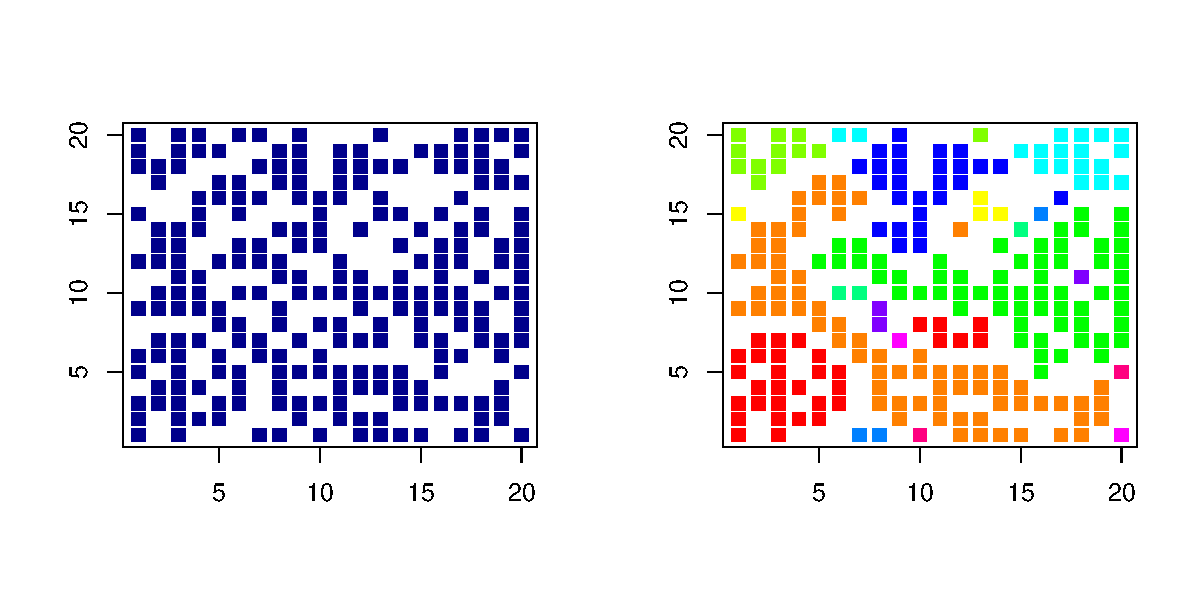
\includegraphics{pics/exdat1.pdf}
\caption{Clustering based on a data frame with a cluster distance equal to the pixel width. Only the four directly connected neighboring cells are joined to a cluster and no diagonal neighbors. The left figure shows the original data and the right figure the clustered result, where each color represent a separated cluster.}
\label{fig:exdat1}
\end{figure}


If we want to use the matrix based version we have first to convert the data into a matrix.

\begin{Schunk}
\begin{Sinput}
> #initiate empty matrix
> exampledata.pop <- matrix(0, nrow=max(exampledata$x), ncol=max(exampledata$y))
> #restructure data
> for(i in 1:NROW(exampledata)){
+   exampledata.pop[exampledata$x[i],exampledata$y[i]] <- exampledata$z[i]
+ }
\end{Sinput}
\end{Schunk}

Afterwards we can call the cca again for the cluster distance s = 1.

\begin{Schunk}
\begin{Sinput}
> example.result <- cca(exampledata.pop, s=1)
> str(example.result)
\end{Sinput}
\begin{Soutput}
 int [1:20, 1:20] 1 0 1 0 0 0 8 8 0 12 ...
\end{Soutput}
\end{Schunk}

The result, example.result, is a matrix that defines for each cell to which cluster it belongs (illustrated by figure \ref{fig:exdat2}). In this example we used the default value 3 for mode, but mode = 1 will have the same effect. However, if mode = 2 all eight neighboring cells would be considered, which would lead to one single cluster. 



\begin{figure}
\centering
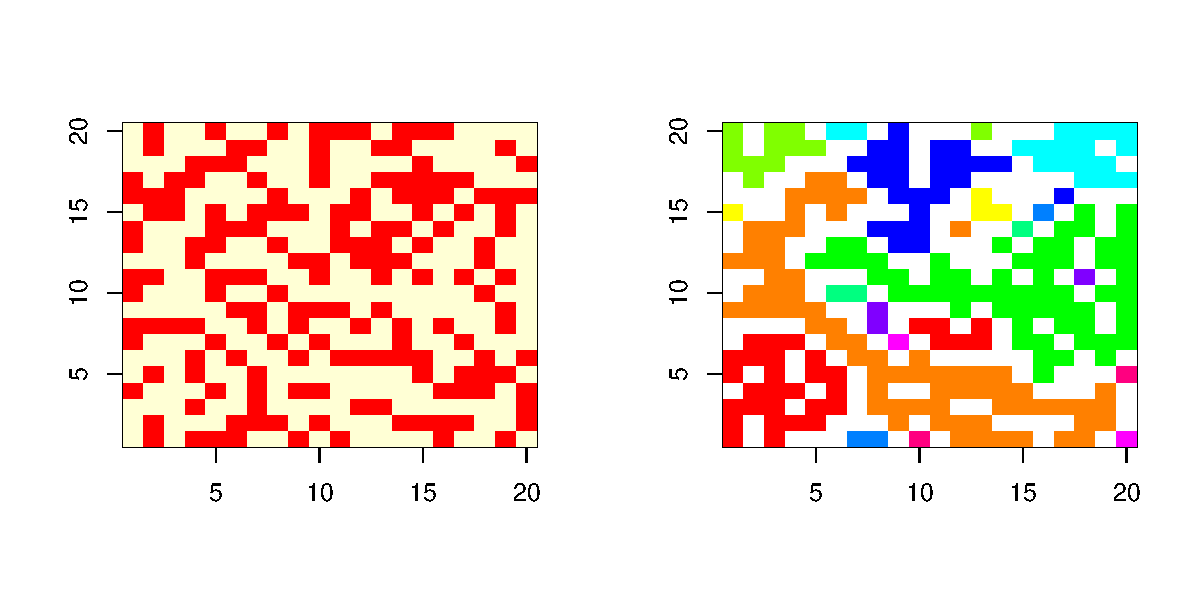
\includegraphics{pics/exdat2.pdf}
\caption{Clustering based on a matrix with a cluster distance equal to the pixel width. The result is exactly the same as the previous result shown in figure \ref{fig:exdat1}.}
\label{fig:exdat2}
\end{figure}



\section{Clustering of geo-referenced data}

The CCA supports native the raster format, but will do the geo-referenced clustering based on points. To do so the cca converts automatically the raster to a data-frame with two columns, namely long and lat coordinates of the center points from the chosen raster cells. For the use of the orthodromic distance, option unit="m", a WGS84 Latitude/Longitude projection of the data is mandatory. The algorithm compares the distances from every cell to each other. If the distance is smaller than the threshold of the cluster-distance the cells will be considered as one cluster.

Let's do a short example: First we will create a raster and then cluster the cells with value one for three different cluster distances 150, 240 and 111 km.

\begin{Schunk}
\begin{Sinput}
> # create a raster and set the projection information
> raster <- raster(extent(0,5,0,5),nrow=5,ncol=5)
> raster[c(1,2,3,5,6,10,17,18,22,23,24)] <- 1
> proj4string(raster) <- CRS("+proj=longlat")
> # get a feeling for the dimensions
> summary(distance(raster)[])
\end{Sinput}
\begin{Soutput}
   Min. 1st Qu.  Median    Mean 3rd Qu.    Max. 
      0       0  111100   65990  111300  157400 
\end{Soutput}
\end{Schunk}

\begin{Schunk}
\begin{Sinput}
> # cluster all cells with value 1
> # for various cluster distances of 150, 240 and 111 km
> cluster <- cca(raster, cell.class=1, s=1.5e+05, unit="m")
> cluster2 <- cca(raster, cell.class=1, s=2.4e+05, unit="m")
> cluster3 <- cca(raster, cell.class=1, s=1.11e+05, unit="m")
\end{Sinput}
\end{Schunk}


Notice the different results, to be more precise the different number of clusters, for the different cluster distances. For the first run with a cluster distance of 150 km where three clusters identified, see figure \ref{fig:raster} left. The distance is large enough to identify all neighbors as part of the cluster. Through an increase to 240 km the upper left cluster and the upper right become one cluster, see figure \ref{fig:raster} middle. The distance is large enough to bridge a horizontal gap of one empty cell, but not to bridge a diagonal gap. This can be reached by a further increase up to 250 km.
A cluster distance smaller than 110 km will result into 11 clusters, every single cell. A special case can be created by choosing a cluster distance of 111 km, see figure \ref{fig:raster} right. In this case the three upper left cells forming one cluster, where as all other cells are separated. This is because of the cell width, which is lower in high latitudes.
It is also possible to cluster a raster pixelwise, without consideration of the projection.
\begin{Schunk}
\begin{Sinput}
> pixel <- cca(raster, cell.class=1, s=1)
\end{Sinput}
\end{Schunk}
\begin{Schunk}
\begin{Sinput}
> str(pixel)
\end{Sinput}
\begin{Soutput}
List of 2
 $ cluster:'data.frame':	11 obs. of  3 variables:
  ..$ long      : num [1:11] 0.5 0.5 1.5 1.5 1.5 2.5 2.5 2.5 3.5 4.5 ...
  ..$ lat       : num [1:11] 4.5 3.5 4.5 1.5 0.5 4.5 1.5 0.5 0.5 4.5 ...
  ..$ cluster_id: num [1:11] 1 1 1 2 2 1 2 2 2 3 ...
 $ size   : num [1:3] 4 5 2
\end{Soutput}
\end{Schunk}
For a clusterdistance equal to the resolution of the raster this will lead to the same result as the in section \ref{sec:first} presented ways or the clump-function from the raster package [2]. The second entry of pixel, the cluster size, is then simple the number of cells for each cluster.



\begin{figure}
\centering
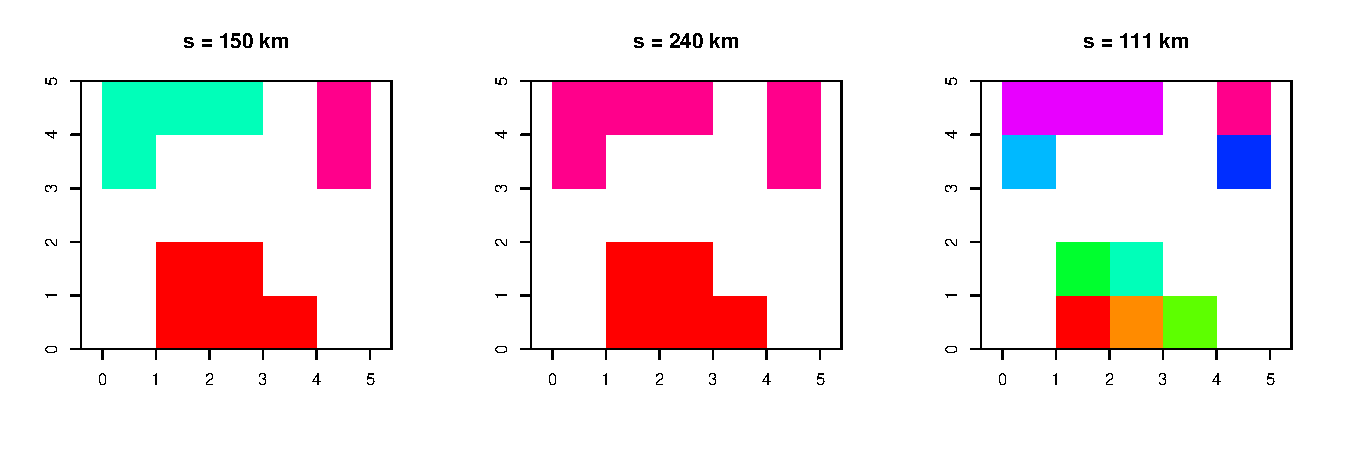
\includegraphics[width=\textwidth]{pics/raster.pdf}
\caption{Clustering of a geo-referenced raster object for several cluster distances. Each colour identifies a cluster. The number of clusters increases with a decrease of the cluster distance.}
\label{fig:raster}
\end{figure}

\subsection{City Clustering}
Another more realistic example for a fictional land-cover data with five different classes, see figure \ref{fig:landcover}. We chose the cell class 1, a cluster distance of 2 km and the unit="m".

\begin{Schunk}
\begin{Sinput}
> data("landcover")
> cities <- cca(landcover, cell.class=1, s=2000, unit="m")
\end{Sinput}
\end{Schunk}

The result, cities, is again a list. However, you can create a raster-object from the results based on the original raster within two lines.

\begin{Schunk}
\begin{Sinput}
> str(cities)
\end{Sinput}
\begin{Soutput}
List of 2
 $ cluster:'data.frame':	116 obs. of  3 variables:
  ..$ long      : num [1:116] 13.3 13.3 13.3 13.2 13.3 ...
  ..$ lat       : num [1:116] 52.2 52.2 52.2 52.2 52.2 ...
  ..$ cluster_id: num [1:116] 1 1 1 1 1 1 1 1 1 1 ...
 $ size   : num [1:9] 17.771 2.449 0.612 1.836 21.398 ...
\end{Soutput}
\begin{Sinput}
> result <- landcover*NA
> result[cellFromXY(result, cities$cluster[,1:2])] <- cities$cluster[,3]
\end{Sinput}
\end{Schunk}

We took the coordinates of the clustered cells to compute the cellnumber and replaced these cells with the corosponding cluster id. The result is shown in figure \ref{fig:landcover}.


\begin{figure}
\centering
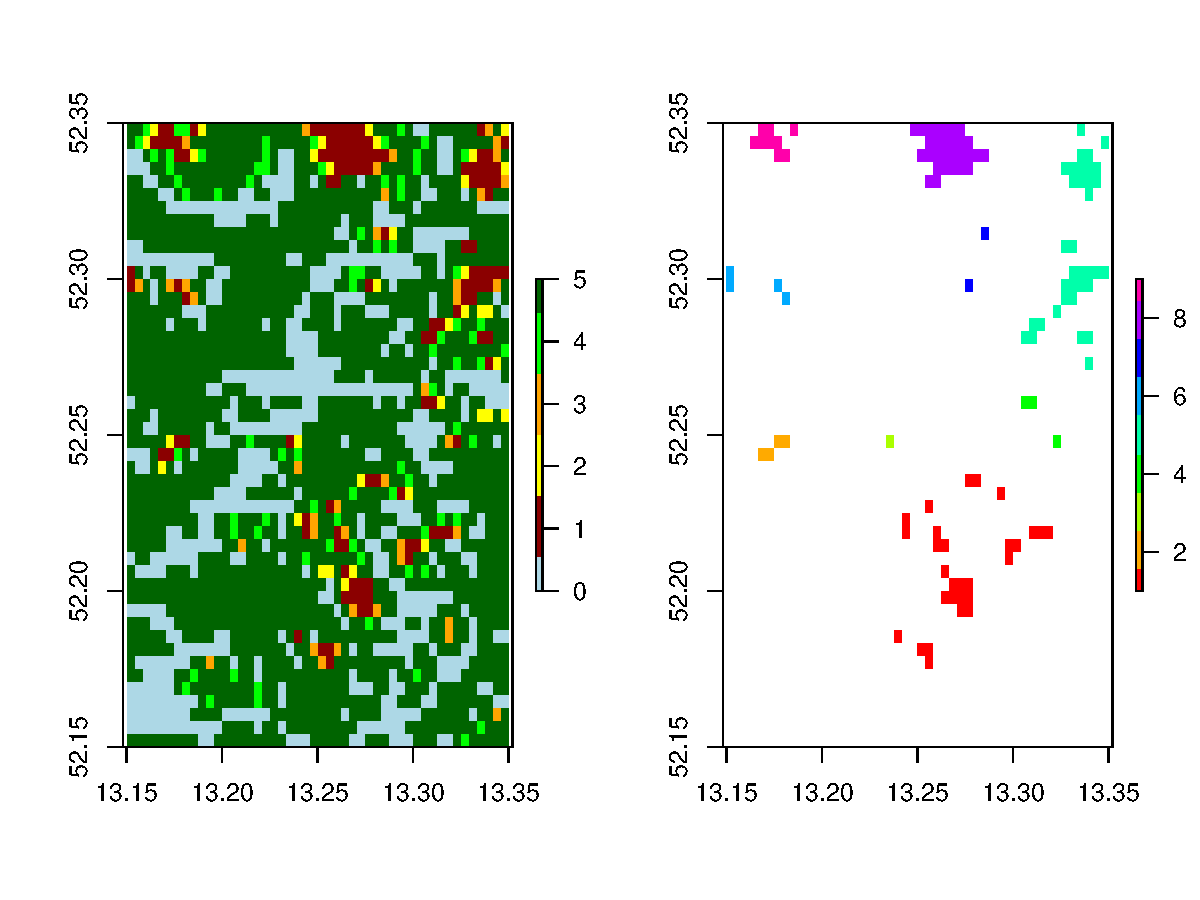
\includegraphics[width=\textwidth]{pics/landcover.pdf}
\caption{Clustering of land cover data. Left side the original data and on the right side the clustered result.}
\label{fig:landcover}
\end{figure}

\subsection{Clustering point data}

\begin{Schunk}
\begin{Sinput}
> library(maps)
> head(world.cities)
> str(world.cities)
\end{Sinput}
\end{Schunk}

\begin{Schunk}
\begin{Sinput}
> city.cluster <- cca(data = world.cities[,c(5,4,1:3,6)], s = 0.5)
\end{Sinput}
\begin{Soutput}
[1] "use as X-coordinates column ' long '"
[1] "use as Y-coordinates column ' lat '"
[1] "Sorting... Done"
[1] "Start Clustering..."
[1] "Clustering... Done"
[1] "Summary... Done"
\end{Soutput}
\begin{Sinput}
> 
\end{Sinput}
\end{Schunk}


\begin{Schunk}
\begin{Sinput}
> city.cluster.m <- cca(data = world.cities[,c(5,4,1:3,6)], s = 56*1e+03,
+                       res.x = 0.05, res.y = 0.05, unit = "m")
\end{Sinput}
\begin{Soutput}
[1] "use as X-coordinates column ' long '"
[1] "use as Y-coordinates column ' lat '"
[1] "Sorting... Done"
[1] "Start Clustering..."
[1] "Clustering... Done"
[1] "Summary... Done"
\end{Soutput}
\begin{Sinput}
> 
\end{Sinput}
\end{Schunk}


\begin{figure}
\centering
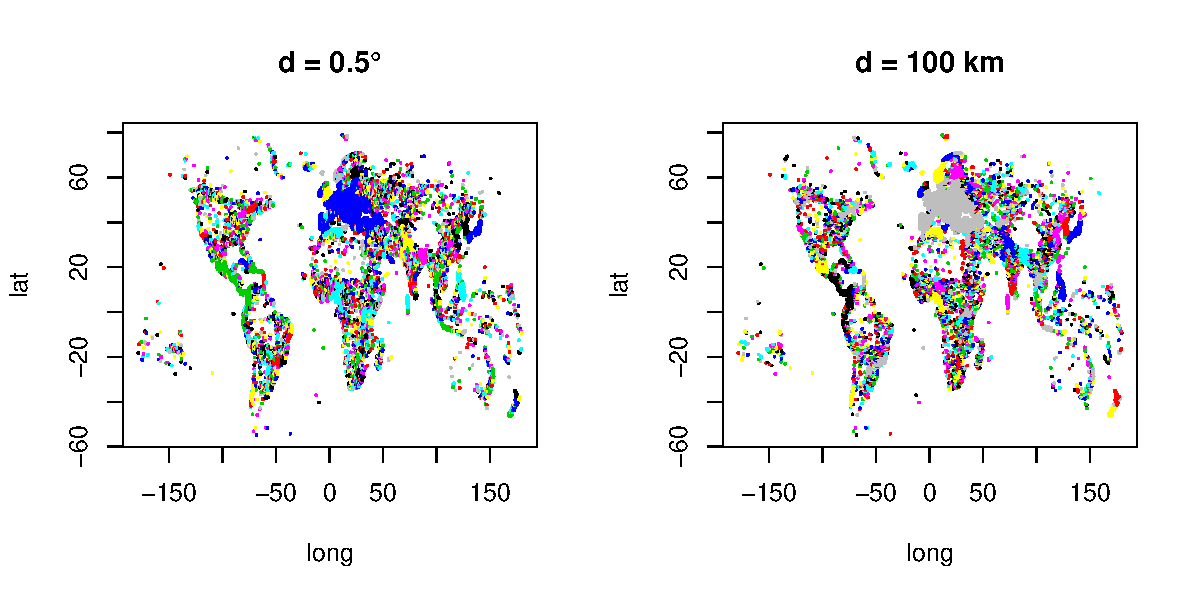
\includegraphics[width=\textwidth]{pics/point_data.pdf}
\caption{CBla bla bla}
\label{fig:landcover}
\end{figure}

\begin{Schunk}
\begin{Sinput}
>   coordinates(city.cluster[[1]]) <- ~long+lat
>   proj4string(city.cluster[[1]]) <- CRS("+init=epsg:4326")
\end{Sinput}
\end{Schunk}

\section{Comparison of the two Versions - matrix vs. list}
\label{sec:compare}

As we have shown already in section \ref{sec:first} the two implemented versions do exactly the same just in different ways. If your data is already in one of the known types (matrix, data.frame, raster) it is logical to use the corresponding implementation of the algorithm. However, there are huge differences in run time and memory consumption which could give you a hint for the right choice.

The memory use of the matrix-based version depends only on the size of the matrix / raster. As for the algorithm two matrices are needed, consequently the memory use will be doubled. For the list-based version the memory needed depends on the number of cells which are occupied. Each of these cells will be saved in a data-frame with xy-coordinates and a placeholder for the cluster id.

To summarize it: The list-version is faster for sparse matrices and large cluster-distances, where as the matrix version is better for dense matrices and small cluster-distances. In general the list version needs less memory.



\begin{figure}
\centering
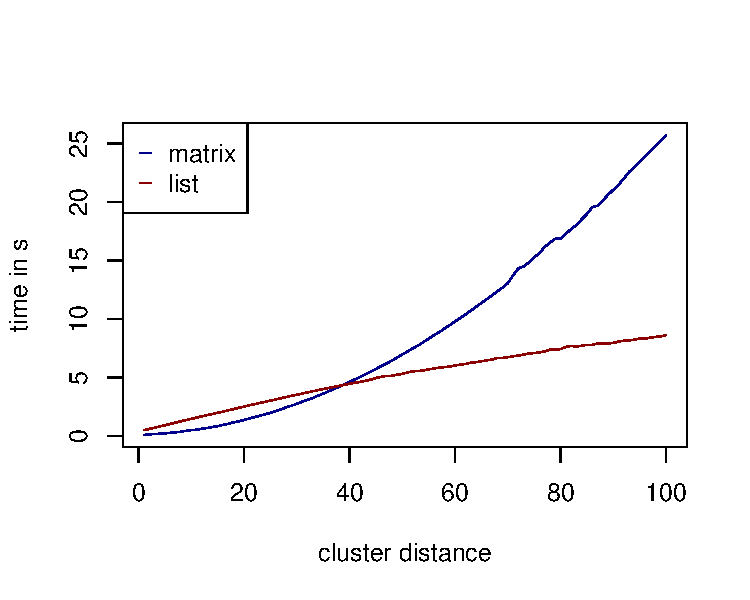
\includegraphics{compare.pdf}
\caption{Comparison of the run time for matrix and list based implementation of the cca.}
\label{fig:compare}
\end{figure}

\newpage
\begin{thebibliography}{9}
\bibitem{Rozenfeld08}
Rozenfeld, H. D., Rybski, D., Andrade, J. S., Batty, M., Stanley, H. E., \& Makse, H. a. (2008). Laws of population growth. Proceedings of the National Academy of Sciences of the United States of America, 105(48), 18702–7. doi:10.1073/pnas.0807435105
\bibitem{raster14}
Robert J. Hijmans (2014). raster: raster: Geographic data analysis and modeling. R package version 2.2-31.
  http://CRAN.R-project.org/package=raster
\end{thebibliography}

\end{document} 
